% ============================================================================
\section{Evaluation Design}
\label{sec:design}
% ============================================================================
\subsection{Properties under Test}
The evaluation tests the four properties named in Section~\ref{sec:intro}, after first validating the instruments that every later number depends on. Table~\ref{tab:evalmap} maps each property to its experiment, data, metrics, and preregistered hypothesis. Experiment E1 tests the expressiveness of the representation, E2 the safety of a single drafted update, E3 the stability of updates applied in a chain, and E4 the detection of affected company policies. E0 validates the instruments, and E5 compares the system with code maintenance and with direct calculation by an LLM.

\begin{table*}[!t]
\caption{Evaluation map: properties, experiments, data, metrics, and preregistered hypotheses. One-sided bounds are 95\% bounds.}
\label{tab:evalmap}
\centering\footnotesize
\setlength{\tabcolsep}{3pt}
\begin{tabularx}{\textwidth}{@{}P{2.7cm} P{0.6cm} P{3.4cm} L P{4.0cm}@{}}
\toprule
Property & Exp. & Data & Metrics & Hypothesis and threshold \\
\midrule
Valid instruments & E0 & four external references, mutants & agreement per observation and per case; mutation score & mutation score $\geq 0.80$ \\
Expressiveness & E1 & 16 unseen changes with 100 examples & representational adaptability (RA): share of changes expressed without engine change & H1: lower bound of RA $\geq 0.70$ \\
Safety of one update & E2 & 13 regulations and 5 labor agreements; 20 distractors & silent error rate (SER), correct application rate (CAR), abstention, selective risk & H2a: upper bound of SER $\leq 0.25$; H2b: CAR above B3 and B4, SER not worse by more than 0.10 \\
Stability of chained updates & E3 & 33 events in order, 150 cases per tax year & operational adaptability rate (OAR); triggered errors; incorrect cases at the end of the chain & H3a: lower bound of OAR $\geq 0.75$; H3b: triggered errors within the noise bound \\
Impact detection & E4 & 134 policy--event pairs & recall, precision, $F_2$ & H4a: lower bound of recall $\geq 0.70$; H4b: $F_2$ above both simple detectors \\
Comparison & E5 & two open-source calculators; 100 operational cases & days and lines of code to adopt TER; exact match of direct LLM calculation & none (descriptive) \\
\bottomrule
\end{tabularx}
\end{table*}

\subsection{Regulation Replay Protocol}
\label{sec:protocol}
The protocol replayed the 13 test events and 20 distractor documents in the order of their issue dates, 33 events in all. Isolated mode (E2) applied each draft to the gold knowledge base before its event. Chained mode (E3) applied each draft to the knowledge base that the system itself had produced. Reusing the drafts of the isolated run gives the transplanted chain, and writing the drafts again with the system's own knowledge base as context gives the regenerated chain. No reviewer intervened in either mode, so the results bound the pipeline from below, and an abstention left the knowledge base unchanged. Each chain ran once and scored 150 sampled cases per tax year, so the number of scored cases grew from 300 to 600 as tax years entered.

\subsection{Data and Temporal Split}
\label{sec:data}
The development set, used to design prompts, gates, and the selection rule, contained 13 regulatory events from 2012 to 2022, five fictional regulations, and one labor agreement. The test set contained the 13 real events of 2023--2026 (Fig.~\ref{fig:timeline}), 20 distractor documents whose correct update is empty, and five real collective labor agreements. It also contained 14 synthetic company policies, four counterfactual versions of real documents with altered values, and 16 unseen changes. Appendix~\ref{app:tables} lists the corpus with the size of each gold update. A news search found no regulation issued between the preregistration and 3 November 2026 that could be used as a prospective test.

The representation and the engine were developed after the test regulations had been published, so hindsight bias weakens the claim that those regulations need no engine change. The 16 unseen changes address this bias. A separate agent wrote them, with 5 to 7 worked examples each, and sealed them with a hash manifest before the representation was frozen. Another agent that took no part in the design then expressed them as updates.

\subsection{Ground Truth and Instrument Validation}
\label{sec:groundtruth}
Every reported number depends on the gold knowledge base $\K^\gold$ and the test cases. Four external references validated both. The first two are the official worked examples in the regulations (GT1), with a holdout opened once, and the PPh 21 calculator of the Directorate General of Taxes (GT2). The other two are 50 cases computed step by step from the regulation texts by a calculator separate from the engine (GT3) and 21 worked examples taken from clauses of the five labor agreements (GT5). Third-party implementations were collected as a fifth reference but not used for validation. Each difference was adjudicated as an error of the knowledge base, an error of the reference, or a legal ambiguity, and ambiguities were settled in 18 written interpretations. A mutation analysis measured whether the test cases detect deliberately altered rules. No human tax practitioner reviewed the gold knowledge base. Its second reader and the reviewers of the gold material were AI agents of the same model family as the model under test.

\subsection{Test Space and Coverage}
The test space holds 2,398 employee-year cases, plus 120 to 180 cases for each company policy. Each tax year has 300 operational cases sampled from provincial wage cells of Statistics Indonesia, 42 to 45 constrained combinations with full pairwise coverage, and 15 cases around the Article 17 bracket boundaries. From 2024, each year adds 321 cases around the TER boundaries. Article 17 boundaries were tested at $b-1000$, $b$, and $b+1000$ because taxable income is rounded down to thousands. Fig.~\ref{fig:coverage} shows the result. All five Article 17 brackets occur, the 35\% bracket only in six boundary cases, and 107 of the 122 TER boundaries are tested. The highest monthly gross in the test space is Rp430.3 million. The TER rates of 30\% to 34\% start at Rp454 million and therefore occur in no case.

\begin{figure}[!t]
\centering
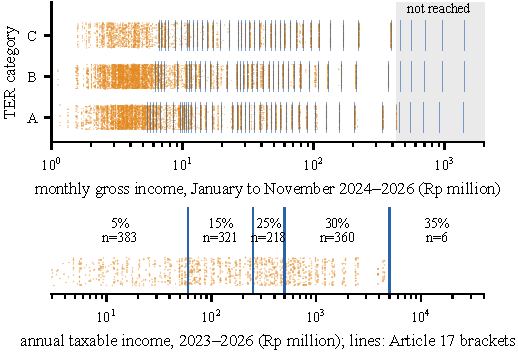
\includegraphics[width=\columnwidth]{figs/fig_coverage.pdf}
\caption{Coverage of the test space. Top: monthly gross income of every non-final TER period by category, with the TER bracket boundaries as lines; the shaded range is not reached. Bottom: annual taxable income against the Article 17 brackets, with the number of cases per bracket (1,110 cases have no taxable income).}
\label{fig:coverage}
\end{figure}

\subsection{Metrics}
\label{sec:metrics}
An update is \emph{correct} when every output value of every test case equals the value of the gold knowledge base to the rupiah at both knowledge dates and the conflict reports agree. One differing value makes it wrong. The strictness follows the use of the numbers, because withholding slips report the tax to the rupiah. Results are counted per observation (one output value of one case at one knowledge date), per tuple (one case at one knowledge date with all its observations), and per case (one employee-year).

The pipeline ends each document in one of three outcomes: a correct update, a wrong update applied without warning (a silent error), or an abstention. SER and CAR are the shares of the first two outcomes over the 18 real documents, and selective risk is SER/(SER + CAR)~\cite{xin2021abstention}. Pass@1, pass@$m$, and 1@$m$ describe the drafts before selection~\cite{chen2021evaluating,li2022alphacode}. RA is the share of unseen changes for which an update reproduces all examples without engine change. OAR is the share of chained events that add no new incorrect case, and the triggered errors of Section~\ref{sec:errortypes} are counted against a noise bound estimated from two independent isolated runs. Impact detection uses recall, precision, and $F_2$ over policy--event pairs, weighting recall because a missed affected policy costs more than a false alarm.

Four exploratory measures were added after the main results. Two describe a wrong update, namely the materiality of each wrong value (exact, within Rp1, within Rp1,000, or larger) and the number of employees it affects. The other two are the element-level precision and recall of a selected update against the gold update and the summed duration of the model calls that drafted an update.

\subsection{Baselines and Ablations}
Two baselines bracket the selection rule. B3 applies the first draft that passes G1 and G2, the pattern of one model call with validation used by single-state formalization~\cite{veeramani2026neurosymbolic,yadamsuren2026formalization}. B4 takes the majority vote of all drafts without gates, the behavioral selection of Gogani-Khiabani et al.~\cite{goganikhiabani2025maintaining}. Two simpler detectors are the baselines for impact detection: B5(i) flags every policy that touches the facts in $F_\Delta$, and B5(ii) scans the text of the policy expressions without the graph. E5 adds two external comparisons, the commit histories of open-source PPh 21 calculators (B1) and an LLM that computes the tax directly from the case data (B2). The ablations remove the knowledge-base context from the prompt, remove each gate in turn or keep only G1, and remove the repair round. Further ablations replace consensus with the first passing draft or with perfect selection, formalize a whole legal state from scratch, and remove SHACL from G1.

\subsection{Statistical Analysis and Preregistration}
Proportions are reported with exact Clopper--Pearson confidence intervals (CIs) and one-sided 95\% bounds. Paired comparisons of CAR use the exact McNemar test with Holm correction, and noninferiority of SER uses the Newcombe CI of the paired risk difference with a margin of 0.10. Each threshold was set at or above the best bound the planned sample can reach; with 18 documents and no error, the exact upper bound of SER is 0.153. McNemar reaches 80\% power with $N = 18$ only for a CAR difference near 0.45, so a failure to reject is not evidence of equivalence. Impact detection uses a bootstrap clustered by event.

The hypotheses, thresholds, data split, main test cases, analysis plan, pipeline, and engine were committed to the public repository (commit \texttt{c5983ff}) before the first test event ran. A git commit is weaker evidence than registration with a third party. The 17 targeted cases of the mutation analysis entered after the first E2 call but before any E2 result was scored. An amendment written after early results (commit \texttt{2df0727}) added the remaining nine distractors, a second isolated run, the regenerated chain, the counterfactuals, the synthetic policies, the ablation without knowledge-base context, a second model, and a sensitivity run with $m = 5$. Apart from the distractors, the second run, and the regenerated chain, the results that rest on the amendment are marked exploratory.

\subsection{Implementation and Cost}
The engine, gates, and pipeline are written in Python, the knowledge graph runs in GraphDB 11.5 with SHACL validation, and the application uses Streamlit. The main model was Claude Opus 5.5, with medium reasoning effort for relevance and high effort for drafting. Its calls used structured JSON output, prompt caching, a limit of 32,000 output tokens, and the provider's default sampling settings. The second model was \texttt{gpt-6.1-sol}. Drafting used $m = 3$ for regulations and $m = 2$ for labor agreements. The experiment calls ran on 28 and 29 October 2026 and were logged in full, so every analysis can be repeated without calling a model. The experiments cost about USD 81.6 for Claude and USD 8.1 for the second model.
